\sectionframe{Decision dependent constraints}
\begin{frame}
 \frametitle{Example: Lewig Wakuxi}
 \begin{figure}
  \centering
  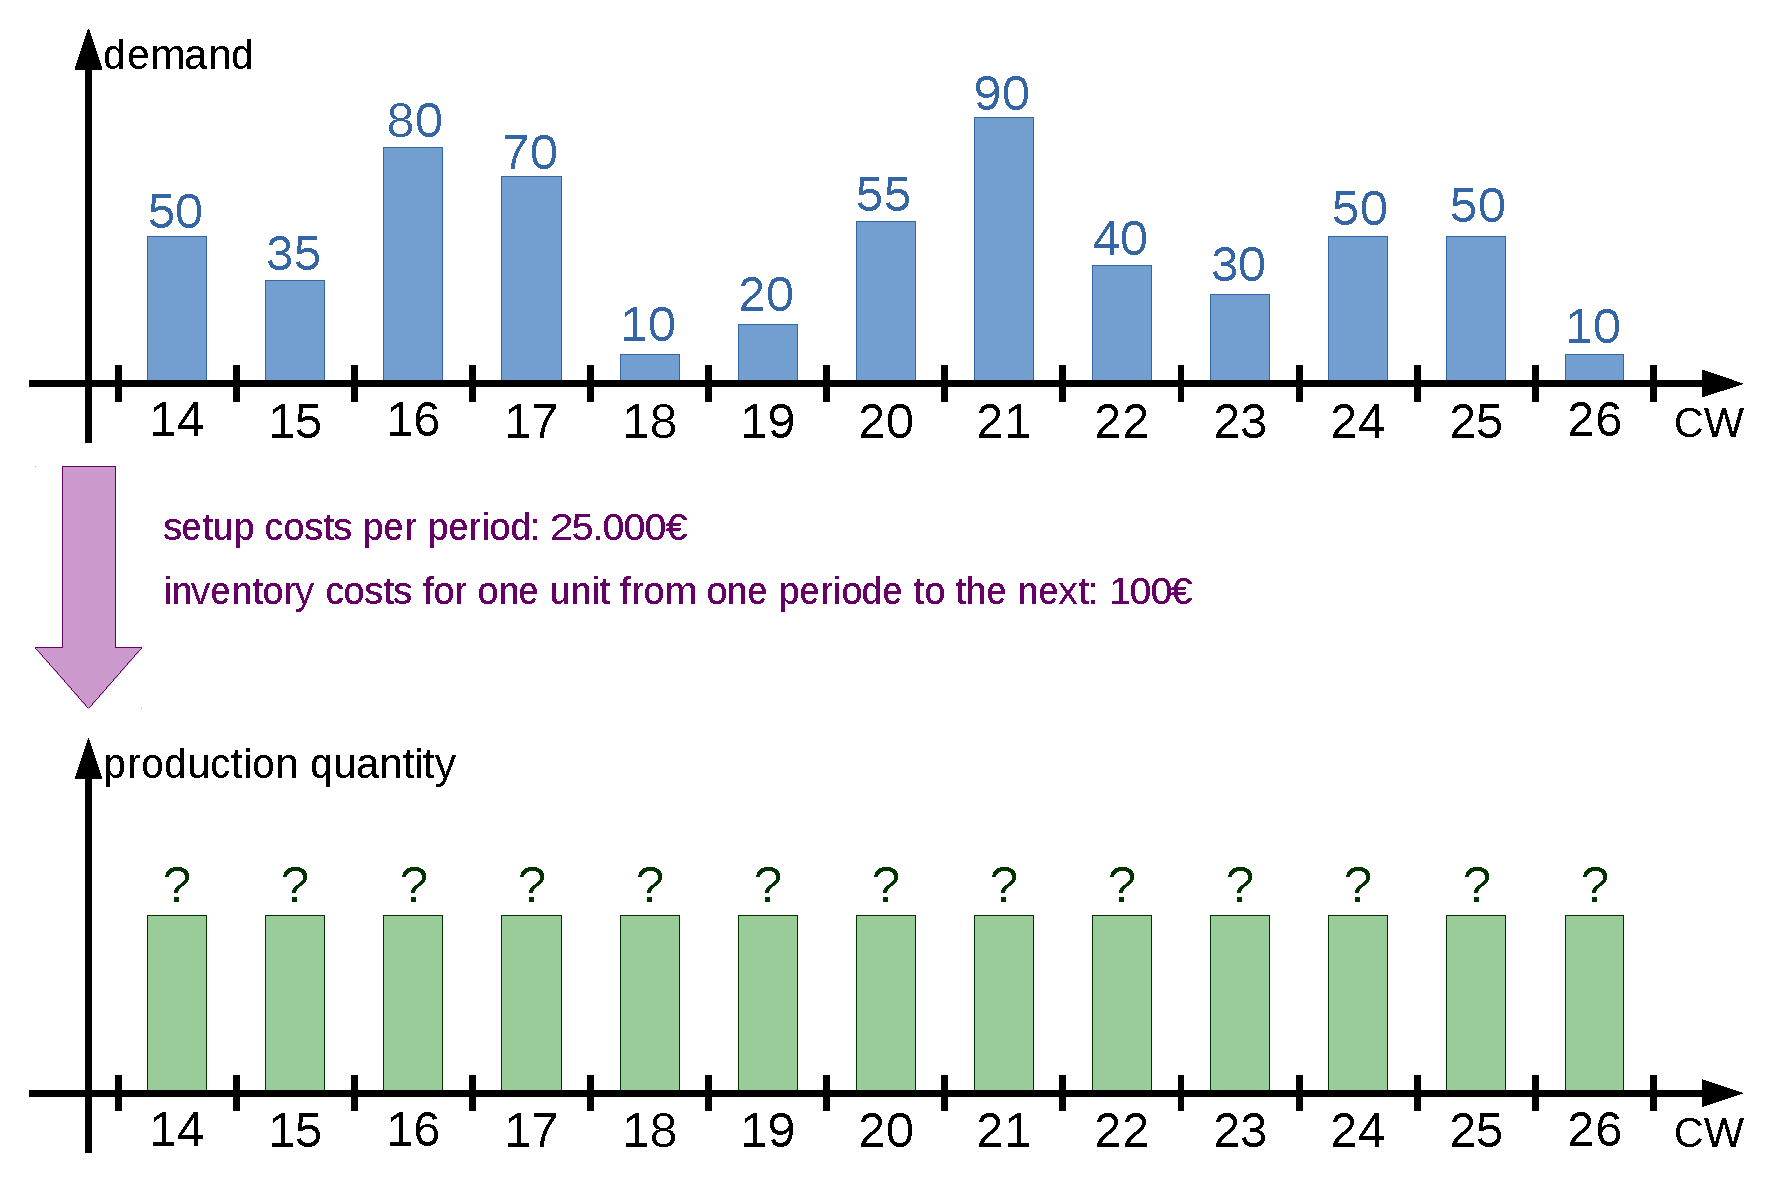
\includegraphics[width=\linewidth]{Bilder/WagnerWhitinProblem}
 \end{figure}
\end{frame}

\begin{frame}\footnotesize
 \frametitle{Model: Wagner-Whitin-problem}
 \begin{tabularx}{\linewidth}{lL}
  \multicolumn{2}{l}{\textbf{Index sets}:}\\
    $T$ & planning periods $\{t_{min}, \ldots, t_{max}\}$\\
  \multicolumn{2}{l}{\textbf{Parameters}:}\\
    $d_t$ & demand in period~$t\in T$\\
    $s_t$ & setup costs in period~$t\in T$\\
    $h_t$ & inventory costs per item in period~$t\in T$\\
    $i_{t_{min}-1}$ & initial inventory\\
    $\alert{M}$ & \mbox{}\alert{a big number}\\
  \multicolumn{2}{l}{\textbf{Decision variables}:}\\
    $x_t$ & production quantity in period~$t\in T$\\
    $i_t$ & inventory at the end of period~$t\in T$\\
    $y_t$ & production decision in period~$t\in T$\\[1ex]
  \multicolumn{2}{l}{\textbf{Model description}:}\\[1ex]
  \multicolumn{2}{l}{
      $
      \begin{array}{rllr}
	\min & \displaystyle\sum_{t\in T} s_t\cdot y_t + h_t\cdot i_t & & \\[3ex]
	s.t. & i_t = i_{t-1}+x_t-d_t & \quad\forall t\in T & \mathrm{(I)}\\
	      & \alert{x_t \leq M\cdot y_t} & \alert{\quad\forall t\in T} & \alert{\mathrm{(II)}}\\
	      & x_t, i_t\geq 0;\;y_t \in \{0,1\} & \quad\forall t\in T & \\
      \end{array}
      $
  }\\[1ex]
 \end{tabularx}
\end{frame}

\subsection{The Big-M-Method}
\begin{frame}
 \frametitle{Die Big-M-Method}
 Let $\mathbf{\overline{x}}$ be the vector of decision variables and $f$ be a linear function. The constraint
  \[
  f(\mathbf{\overline{x}}) \leq b\qquad\text{bzw.}\qquad f(\mathbf{\overline{x}}) \geq b
  \]
  shall only be constraining if a decision represented by the binary variable~$y$ has been made.

  \begin{block}{Decision dependent constraint}
  Let $M$ be a sufficiently big number.\\
  $f(\mathbf{\overline{x}}) \leq b$ \quad\textrightarrow{}\quad $f(\mathbf{\overline{x}}) \leq b + M\cdot y$\\
  $f(\mathbf{\overline{x}}) \geq b$ \quad\textrightarrow{}\quad $f(\mathbf{\overline{x}}) \geq b - M\cdot y$
\end{block}
\end{frame}

\subsection{OPL: modeling of time periods}
\begin{frame}
 \frametitle{Problem with implementation of time periods}
 \begin{block}{Constraint of example "`Lewig Wakuxi"'}
 $i_t = i_{t-1}+x_t-d_t \qquad\forall t\in T \qquad \mathrm{(I)}$
 \end{block}
 \begin{minipage}[t][15ex]{\linewidth}
 \only<1>{\begin{block}{Implementation try 1}\ttfamily\scriptsize
 \{string\} T = \{"KW14", "KW15", "KW16", "KW17"\};\\
 dvar float+ i[T];\\
 \mbox{}\quad forall(t in T) i[t] == i[\alert{t-1}] + x[t] - d[t];
 \begin{flushleft}\sffamily
  
\includegraphics[height=2ex]{Bilder/error-icon}{} Operator for string - int not available.
 \end{flushleft}
 \end{block}}
 \only<2>{\begin{block}{Implementation try 2}\ttfamily\scriptsize
 \{int\} T = \{14, 15, 16, 17\};\\
 dvar float+ i[T];\\
 \mbox{}\quad forall(t in T) i[t] == i[\alert{t-1}] + x[t] - d[t];
 \begin{flushleft}\sffamily
  
\includegraphics[height=2ex]{Bilder/error-icon}{} Index out of bound for array "{}i"{}: 13.
 \end{flushleft}
 \end{block}}
 \only<3>{\begin{block}{Implementation try 3}\ttfamily\scriptsize
 \{int\} T = \{14, 15, 16, 17\};\\
 \{int\} T0 = \{13, 14, 15, 16, 17\};\\
 dvar float+ i[T0];\\
 \mbox{}\quad forall(t in T) i[t] == i[t-1] + x[t] - d[t];
 \end{block}}
 \only<4>{\begin{block}{Implementation try 4}\ttfamily\scriptsize
 int Tmin = 14; \\
 int Tmax = 17;\\
 range T = Tmin..Tmax; \\
 dvar float+ i[Tmin-1..Tmax];\\
 \mbox{}\quad forall(t in T) i[t] == i[t-1] + x[t] - d[t];
 \end{block}}
 \end{minipage}
\end{frame}

\subsection{Disjunctive Constraints}
\begin{frame}
 \frametitle{Disjunctive Constraints I}
 A model shall have to following constraints:
 \begin{align*}
  &f(\mathbf{\overline{x}}) \leq b\\
  &g(\mathbf{\overline{x}}) \leq d
 \end{align*}
 It is enough to only fullfil one constraint.
 
 \begin{block}{Disjunctive Constraints}
 Let $M$ be a sufficiently large number and $y$ be a binary auxiliary variable.
 \begin{align*}
  &f(\mathbf{\overline{x}}) \leq b + M\cdot y\\
  &g(\mathbf{\overline{x}}) \leq d + M\cdot (1-y)
 \end{align*}
 \footnotesize $\geq$-constraint analog
 \end{block}
\end{frame}

\begin{frame}
 \frametitle{Disjunctive Constraints II}
 A model shall have to following constraint:
 \begin{align*}
  &g(\mathbf{\overline{x}}) \leq d
 \end{align*}
 This constraint only needs to be fullfiled if it holds:
 \begin{align*}
  &f(\mathbf{\overline{x}}) > b
 \end{align*}
 
 \begin{block}{Disjunctive Constraints}
 Let $M$ be a sufficiently large number and $y$ be a binary auxiliary variable.
 \begin{align*}
  &f(\mathbf{\overline{x}}) \leq b + M\cdot y\\
  &g(\mathbf{\overline{x}}) \leq d + M\cdot (1-y)
 \end{align*}
 \footnotesize $\geq$-constraint analog
 \end{block}
\end{frame}
